% vim: set fileencoding=utf-8 encoding=utf-8:
\documentclass[spanish]{article}
\usepackage{babel}
\usepackage[utf8]{inputenc}
\usepackage{fullpage}
\usepackage{url}
\usepackage{palatino}
\usepackage{mathpazo}
\usepackage{amsmath}
\usepackage{amssymb}
\usepackage{graphicx}

\newcommand{\choquet}{\mathcal{C}\mspace{-18mu}\int}

% set members for example
\newcommand{\SMA}{\square}
\newcommand{\SMB}{\spadesuit}
\newcommand{\SMC}{\heartsuit}
\newcommand{\SMD}{\clubsuit}
\newcommand{\SME}{\diamondsuit}


\title{Reconocimiento de Patrones\\Discusión del artículo \textit{Similarity~Measures}}
\author{Roberto Bonvallet \\ \url {<rbonvall@gmail.com>}}
\date{Noviembre de 2008}

\begin{document}
\maketitle

\section{Resumen}
El artículo \textit{Similarity Measures}~\cite{sim} aborda el problema de medir
disimilaridades en espacios de características, desde el punto de vista de los
requerimientos de un sistema de recuperación de información.


\section{Modelos axiomáticos presentados en el artículo}
El artículo presenta cuatro modelos axiomáticos de similaridad, los que son caracterizados por 
la representación de los estímulos y por las propiedades que cumplen las funciones de similaridad.
Estas propiedades están definidas en el espacio de características y no en un espacio psicológico,
por lo tanto no son necesariamente verificables a través de experimentos.

La relación entre un espacio sicológico y un espacio de características está dada por una ley de
generalización.  El criterio que debe satisfacer una ley de generalización es que la probabilidad
que un estímulo $S_i$ gatille una respuesta asociada a otro estímulo $S_j$ decaiga exponencialmente
con respecto a la distancia en el espacio de características~\cite{shepard}.  En general, se supone
que la distancia sicológica es $\delta = g\circ d$, donde $g$ es una función que satisface este
criterio y se denomina función de generalización.

\subsection{Axiomas métricos}

\begin{description}
    \item [Autosimilaridad constante:]
        $d(A, A) = d(B, B)$;
    \item [Minimalidad:]
        $d(A, B)\ge d(A, A)$;
    \item [Simetría:]
        $d(A, B) = d(B, A)$;
    \item [Desigualdad triangular:]
        $d(A, B) + d(B, C)\ge d(A, C)$.
\end{description}
Muchos modelos de similaridad suponen que el espacio subyacente cumple con estos axiomas,
pero su validez es cuestionada por dos motivos:
\begin{itemize}
    \item experimentos de percepción humana han arrojado resultados
        inconsistentes con el modelo; y
    \item la desigualdad triangular no es verificable experimentalmente,
        pues no se traduce en una propiedad similar para la similaridad juzgada.
\end{itemize}


\subsection{Estructura de proximidad monótona}
La estructura de proximidad monótona es un modelo diseñado para ser verificable experimentalmente.
Esto se logra imponiendo propiedades de tipo ordinal, cuya satisfacción no es alterada por la función de
generalización.  Este modelo es más general y menos restrictivo que el métrico, y otorga
más importancia al cumplimiento de propiedades a lo largo de los ejes.  Las propiedades son:
\begin{description}
    \item [Dominancia:]
        análoga a la desigualdad triangular, pero a lo largo de los ejes.
    \item [Consistencia:]
        el orden a lo largo de una dimensión es independiente de otras
        dimensiones~(ver figura~\ref{fig:comparacion}).
    \item [Transitividad:]
        el traslape de trios ordenados a lo largo de una dimensión implica
        que los cuatro puntos involucrados están ordenados.
\end{description}
Además, se propone una cuarta propiedad con el fin de discriminar modelos
diferentes:
\begin{description}
    \item [Desigualdad de esquina:] XXX
\end{description}



\subsection{Modelo de contraste de características}
En el modelo de contraste de características~(FCM), el espacio de características está formado por
conjuntos de características binarias, que un estímulo puede tener o no.
\begin{description}
    \item [Calce:] la similaridad tiene la forma $s(a, b) = F(A\cap B, A-B, B-A)$.
    \item [Monotonía:] la similaridad está influenciada por el traslape de características comunes;
        por ejemplo, en el siguiente ejemplo $A$ se parece más a $B$ que a $C$:
        \begin{align*}
            A &= \{\phantom{\SMA,  \SMB,} \SMC,          \SMD,          \SME\}  \\
            B &= \{\phantom{\SMA,} \SMB,  \SMC,          \SMD\phantom{, \SME}\} \\
            C &=          \{\SMA,  \SMB,  \SMC\phantom{, \SMD,          \SME}\}
        \end{align*}
    \item [Independencia:] el orden entre pares de estímulos que concuerdan en
        dos de los componentes de la propiedad de calce es independiente ante
        cambios en la tercera componente~(ver figura~\ref{fig:comparacion}).
\end{description}
Un resultado importante acerca este modelo es el teorema de representación: si una función de
similaridad $s$ satisface las tres propiedades, existe una función de similaridad $S$ de la forma
$S(a, b) = f(A\cap B) - \alpha f(A-B) - \beta f(B-A)$, que es equivalente a $s$ en el sentido que
preserva el orden entre pares de estímulos.  La función $f$ se denomina la \emph{saliencia} de un
estímulo.

\begin{figure}[t]
  \centering
  %\includegraphics%
  %    [width=0.8\textwidth]%
  %    {imagenes/comparacion.png}
  \caption{\small %
    Comparación entre las propiedades de consistencia, de la estructura de
    proximidad monótona, e independencia, del FCM.  Ambas describen
    características compartidas entre pares de puntos que permiten asegurar que el
    orden se conserva al cambiar otra característica.  En el primer caso, se
    estas características son dimensiones del espacio; en el segundo, son las
    componentes en que concuerdan los pares de estímulos.
  }
  \label{fig:comparacion}
\end{figure}

\subsection{FCM difuso con dependencia de características}
El FCM difuso es una extensión del FCM en que las características binarias (que un estímulo puede
tener o no) son reemplazadas por un conjunto de predicados difusos, cada uno de los cuales el
estímulo satisface en cierta medida $\mu_i$.  La representación de un estímulo es el conjunto
ordenado $\mu = \{\mu_1, \ldots, \mu_n\}$.  Esta extensión permite la incorporación de
características numéricas.

Un resultado similar al teorema de representación se cumple en el caso difuso, como se demuestra en
el artículo.  Tras definiciones apropiadas de los operadores difusos de intersección y diferencia de
conjuntos, $\mu_\cap$ y $\mu_-$, la función de similaridad de Tversky se define como:
\begin{equation}
    S(\phi, \psi) = \sum_i\bigl[\mu_\cap (\phi_i, \psi_i) -
                          \alpha\cdot\mu_-  (\phi_i, \psi_i)   -
                          \beta \cdot\mu_-  (\psi_i, \phi_i)\bigr],
\end{equation}
en la que se ha utilizado la cardinalidad $\#\mu = \sum_i\mu_i$ como función de saliencia.

En el artículo, los autores proponen una extensión del modelo para dar cuenta de la
interacción de características, de modo que el grado de verdad de una característica pueda afectar
la medida del conjunto completo de características.  La saliencia $f(\mu) = \#\mu$ es
generalizada en la forma de una integral de Choquet~(ver figura~\ref{fig:choquet}):
\begin{equation}
    f(\mu) = \sum_i\mu_i = \sum_i\mu_{(i)}
           = \sum_i \bigl(\mu_{(i)} - \mu_{(i-1)}\bigr)
             \underbrace{\frac{n-i+1}{n}}_{m\bigl(\{\mu_{(i)}\}\bigr)}
           = \choquet \mu\;m,
    \label{choquet}
\end{equation}
donde $m: 2^\mu\to{}[0, 1]$ es una medida del aporte a la saliencia total de un subconjunto de
características, y que en general debe satifacer
$m(\varnothing)=0$,
$m(\mu)=1$ y
$m(A\subseteq B)\leq m(B)$.  En el caso particular de la ecuación~\ref{choquet}, $m$ además es aditiva y
equidistribuida.

\begin{figure}[t]
  \centering
  \includegraphics%
      [width=0.8\textwidth]%
      {imagenes/croquet.png}
  \caption{\small %
    A la izquierda, la saliencia de un estímulo vista como una integral de Choquet.
    Las diferencias en grado de verdad entre características consecutivas
    aportan a la saliencia en la medida del conjunto asociado.
    A la derecha, el aporte a la saliencia al haber dependencias
    está dada por el área punteada.  Según este modelo,
    los predicados no son más o menos ciertos por la influencia de otras
    características, sino que sólo cambia la medida en que aportan a la
    saliencia total.
  }
  \label{fig:choquet}
\end{figure}

La dependencia entre dos características $x_h$ y $x_k$ es modelada alterando la aditividad de $m$
con un término adicional:
\begin{equation}
    m\bigl(\{x_h, x_k\}\bigr) =
    m\bigl(\{x_h\}\bigr) +
    m\bigl(\{x_k\}\bigr) +
    \gamma_{hk} m\bigl(\{x_h\}\bigr) m\bigl(\{x_k\}\bigr),\qquad\gamma_{hk}\ge0.
\end{equation}
Los coeficientes $\gamma_{i_{j_1}\ldots i_{j_p}}$ caracterizan unívocamente la medida, 
y deben ser determinados experimentalmente.  Además, deben satisfacer las propiedades para que $m$
sea una medida válida.

Dada una medida $m$ que incorpora las dependencias, la similaridad de Tversky en el modelo extendido
se define como:
\begin{equation}
    S(\phi, \psi) = \choquet\bigl[\mu_\cap (\phi, \psi) -
                            \alpha\cdot\mu_-  (\phi, \psi)   -
                            \beta \cdot\mu_-  (\psi, \phi)\bigr]\;m.
\end{equation}



\section{Medidas de similaridad y recuperación de información}
Del artículo se puede rescatar varios requerimientos y criterios que debe cumplir un sistema de
recuperación de información, y que deben traducirse en propiedades de las medidas de similaridad
escogidas.  Estas propiedades no son satisfechas por los axiomas métricos, y son el punto de partida
en la exploración de alternativas.

\subsection{Similaridad consulta-resultado en vez de punto-punto}
Como las consultas y los resultados son representados como puntos en un
mismo espacio de características, la medida de similaridad debe tomar en cuenta
la naturaleza diferente de ambos elementos.  La consecuencia más importante de
esto, y que resulta poco intuitiva en un comienzo, es la violación del axioma de
simetría en un espacio métrico.  Este fenómeno es el que se denomina
\emph{saliencia} de un estímulo, y tiene que ver con la manera en que se desea
interpretar el estímulo: como una consulta (esbozo incompleto) o como un resultado.

Un ejemplo cotidiano es la relación que existe entre una búsqueda web, p.ej.
Google, y la relevancia de los resultados obtenidos.  Si uno busca la palabra
«perro», uno estaría satisfecho al obtener como resultado un artículo de mil
palabras sobre «cuidados del perro».  Pero si uno utiliza como patrón de
búsqueda el artículo entero, uno no esperaría obtener como respuesta simplemente
la palabra «perro».

\subsection{Correlación con la similaridad perceptual}
Una usuaria de un sistema de recuperación de información espera resultados
que ella considera relevantes para la búsqueda que realizó.  El hecho que la
similaridad sea medida en un espacio de características subyacente no es
importante para ella.

Los axiomas métricos fallan tanto experimentalmente como teóricamente en este
sentido:  cada uno de ellos ha sido violado en experimentos de percepción, y la
desigualdad triangular no es verificable bajo el supuesto de una ley de
generalización monótona.

Por otra parte, la estructura de proximidad monótona es un modelo diseñado para
ser verificable por la vía experimental.  Además, el FCM difuso con dependencias
tiene parámetros que deben ser determinados en experimentos.

\subsection{Verificabilidad experimental}
Como consecuencia del ítem anterior, es imprescindible que un modelo axiomático
sea verificable a través de experimentos de percepción, ya que ésta es la única
manera de medir la similiaridad perceptual.

XXX


\subsection{Importancia del ordenamiento de los resultados}
El principal rol de una medida de similaridad es imponer un ordenamiento de los
resultados de acuerdo a su relevancia respecto a la consulta.  El valor preciso
de la similaridad no es tan importante.

Una ventaja práctica de esto es que permite simplificar modelos complicados,
manteniendo como única condición que el orden sea conservado.  En el caso del
modelo de contraste de características, esta propiedad se manifiesta en el
teorema de representación, que permite introducir una nueva similaridad basada
en la saliencia.

\subsection{Relevancia de las características por separado}
La noción de distancia en un espacio euclideano es esencialmente isotrópica: los
ejes coordenados no tienen ninguna relevancia por sí solos.  La isotropía es
consecuencia de los axiomas, y resulta ser una exigencia demasiado restrictiva
para proponer medidas de similaridad alternativas.

Perceptivamente, las características sí tienen importancia por sí
solas, y direcciones arbitrarias en el espacio de características no tienen
un significado inherente para una persona.  Los modelos presentados sí reflejan
esta distinción.

Por otra parte, si bien las características no se combinan arbitrariamente en el
espacio, sí existen dependencias entre ellas.  El FCM difuso extendido da cuenta
de estas dependencias de manera explícita en la función de similaridad, sin
necesidad de imponer propiedades sobre el espacio de características.


%\section{Comparación entre los modelos}


%\begin{figure}[t]
%  \centering
%  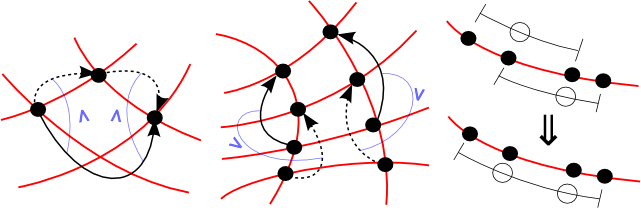
\includegraphics[bb=0 0 513 166]{imagenes/dom-cons-trans.png}
%  % dom-cons-trans.png: 641x208 pixel, 90dpi, 18.09x5.87 cm, bb=0 0 513 166
%  \caption{\small %
%    Ejemplos de las propiedades de un espacio con estructura de proximidad
%    monótona. Las líneas con flechas representan distancias entre puntos del
%    espacio de características.
%    (a) Dominancia: distancia diagonal es mayor que a lo largo de cada eje.
%    (b) Consistencia: las relaciones de orden a lo largo de una dimensión son
%        independientes de otras dimensiones.
%    (c) Transitividad: relaciones de orden traslapadas fuerzan las mismas
%        relaciones entre los puntos en la región de traslape.
%  }
%  \label{fig:cons-dom-trans}
%\end{figure}

\begin{figure}[t]
  \centering
  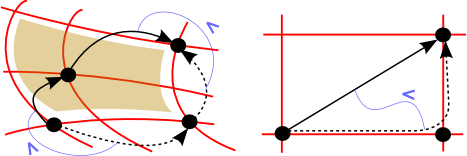
\includegraphics[width=0.8\textwidth]{imagenes/esquina.png}
  % esquina.png: 467x156 pixel, 90dpi, 13.18x4.40 cm, bb=0 0 374 125
  \caption{\small %
    Comparación entre la desigualdad de esquina y la desigualdad
    triangular.  La desigualdad triangular compara la distancias directa con
    la distancia a lo largo de dimensiones entre dos puntos.  La desigualdad de
    esquina sólo impone estas restricciones por tramos, pero deben cumplirse
    para cualquier lugar de la zona sombreada donde esté el punto central.
  }
  \label{fig:esquina}
\end{figure}




%\begin{thebibliography}{1}
\begin{thebibliography}{99}
    \bibitem{sim}
        Simone Santini, Ramesh Jain.
        \emph{Similarity Measures.}
        IEEE Trans.~on Pattern Analysis and Machine Inteligence.
        Vol.~21, No.~9, September~1999.
    \bibitem{shepard}
        Roger~{}N.~Shepard.
        \emph{Toward a Universal Law of Generalization for Physical Science.}
        Science, vol.~237, pp.~1317--1323, 1987.
\end{thebibliography}

\end{document}
